%%% Local Variables: 
%%% mode: latex
%%% TeX-master: "../main"
%%% End: 

\chapter{书面翻译}
\begin{center}
\section*{基于安卓平台设计和实现的医患交互系统$^{[1]}$}
\end{center}

摘要-医疗服务的信息化已经成为了国际发展的一个趋势。随着信息技术的迅速发展,越来越多的医院为了改善医疗服务而加速了基于信息平台的整体服务的实现。移动互联网的发展为医药产业提供了全新的服务模式和发展方向。安卓是一个基于Linux平台开源的移动手机操作系统。因为它的开放性和便捷的开发方式,它在移动互联网的领域上有很高的地位。在这篇文章中,我们展现了一个基于安卓的医患交互系统。它在移动终端上出色的表现让病人能通过连接医院的服务器获取到关于病症建设性的意见,他们也可以通过这个交互系统和医生进行交流,同时医生们也可以在任何时刻、任何地点通过呈现在这些硬件移动终端上的数据跟踪病人的情况从而作出及时的诊断。

关键词:安卓;移动健康;移动互联网;移动定位


\section*{1. 介绍}

医患交互系统的建立和发展对于现在的医疗服务信息化来说是相当重要的需求,尤其是移动交流技术飞速发展的今天,移动互联网的诸多有点都能购被充分利用在弥补医生和病人之间时间和地理位置的差别从而提供快速、充足的医药服务,从而它已经成为了衡量一个医院是否有竞争力的重要指标。通过移动终端和专业服务的连接,医生和病人都能通过比传统更好的交互方式获取到数据。安卓是一个基于Linux平台的开源操作系统,它主要用于移动设备,它良好的性能使它的使用市场不断扩大。同时,网络应用和数据库技术这两个平台也正在逐渐地成熟,因此借助这些平台我们可以在安卓上开发一个医患交互系统去满足医生能更便捷和方便地治疗病人、和病人沟通的需求$^{[2]}$。

\section*{2. 安卓和移动健康}

HIMSS(医疗信息和管理系统安全)给出过关于移动健康的确切定义:即通过移动交互技术比如平板,手机和卫星系统来提供医疗服务或信息。随着现代移动技术的迅速发展,移动健康的规模和服务质量都在提升。为了开发一套方便的医患交互系统,使用成熟的集成终端平台已经变成了刚需。安卓的诞生给我们提供了很多便捷。

\subsection*{2.1 关于安卓}

安卓由操作系统、中间件、用户界面和应用软件组成$^{[3]}$。它开源的特性使得这个平台能够更快地发展新技术、有新创新,也让我们能够很容易地定制个性服务。在安卓上开发一个医患交互系统因为其市场地开放性能够有很好地商业前景、也能够很大程度上增加服务的竞争性。

\begin{figure}[h]
  \centering
  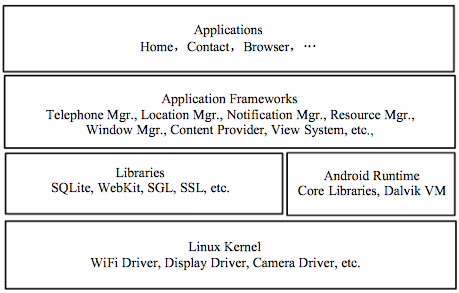
\includegraphics[clip]{paper-1}
  \caption*{图~1\hskip1em 安卓系统结构}
\end{figure}

\subsection*{2.2 关于移动健康}

近几年,移动健康成为了电子健康(指的是用信息交流技术如电脑,手机和卫星提供医药服务和信息)领域的重要分支。随着低成本的移动手机和全球流行化的移动互联网,成千上万曾经购买不起固定电话或电脑网络的人现在能够将手机作为一种日常交流和数据传输的工具,这也为使用移动技术来支持医药服务打下了扎实的奠基。

随着移动交互技术的发展,越来越多的服务能够更正规、快速和廉价得传播。网络带宽的变大、覆盖面的变广给为移动健康开发更好、更合适的应用提供了好的基础。

\section*{3. 系统设计}

我们提出的系统包括两个类型:医生用户和病人用户,这个系统也包括以下这些特征:症状和处方的查询,医患间非实时的通讯,病人地理位置,病人信息的监控。

\subsection*{3.1 症状和处方的查询}

在这里会运用一些缩写和简写。缩写不包括IEEE,SE,MKS,CGS,sc,dc和rms。在标题中会尽量不要使用缩写(除非不可避免)。

1) 原理分析:这个子模块是为了病人能够得到便捷的服务而设计的。一般得了小毛小病的病人能够通过这个服务访问医院的数据库以查看症状有关的信息和推荐的养生之道来达到自我检查的目的,这样可以节省病人和医生很多的时间和精力。

为了设计这个自模块我们需要同时考虑移动终端和用户行为的资源是有限的。首先,查询动作的周期应该越短越好,所以我们应该为用户提供很好的字典结构使得用户能够快速准确地获取查询地结果。其次,考虑到信息内容储存和表达应该达到最优的性能,移动终端应该以最快的速度根据性能的限制给用户展现查询结果。第三,移动终端应该能够直接支持HTML和XML以防止在信息传递的过程中用以查询结果的服务器返回的信息缺失一些内容导致整个原始内容的丢失。

2) 模块设计:首先我们需要在医院服务器上建立一个医药方法信息的数据库。临床疾病的分类、症状和治疗方案应该都需要存储在数据库平台里。关系数据库里应该为病人的查询包括主要器官的病理学、症状和治疗方案、建议的疗养方法的数据。

在移动终端设备上,我们用集成的数据库系统SQLite1.3来备份移动数据$^{[3]}$来保证系统在离线时也能整场运行。SQLite时一个开源的集成的数据库引擎。它能完全独立地提供几乎所有SQ192标准并且在所有主要地操作系统上运行。数据的一致性和扩展性应该通过同步移动端备份的数据和中央数据库而被保证的。这个系统使用SyncML协议在开源的funambol工程框架上做二阶开发$^{[4]}$。

\begin{figure}[h]
  \centering
  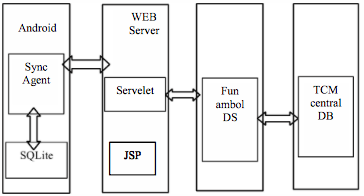
\includegraphics[clip]{paper-2}
  \caption*{图~2\hskip1em 数据同步自模块结构}
\end{figure}

\subsection*{3.2 医患间非实时通讯}

1) 原理分析:和医生的交流能够给病人更好的服务体验。即时通讯需要医生一直在线,然而这在医药界是不太合理的,所以非实时应该是医患交流的主要模式,也就是,病人能够在系统中留言或者提问,而医生也能够通过系统来回答这些问题。

目前的信息交换平台主要基于类似BBS的网页刷新机制,然而这样的传输方式的缺点在于数据量大,使得要消耗很多的流量,所以这不适合于移动终端的信息交流。非实时交流不仅强调信息的重要性,也强调回复操作能够方便和快速。因此最好的方式是结合互联网和常用的交流方式,比如传统新建。

2) 模块设计:在安卓平台上设计一个电子邮件系统需要系统直接支持POP3协议接受邮件、SMTP来发送邮件。这样可以解决传统手机靠短信传递信息的不方便和慢速,但前提是协议的回话以及用户在连续的网络环境里。移动医疗应该支持手机间的电子邮件通讯。这个电子邮件系统的框架可以见图3。

\begin{figure}[h]
  \centering
  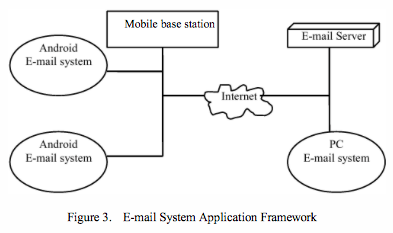
\includegraphics[clip]{paper-3}
  \caption*{图~3\hskip1em 邮件应用系统框架}
\end{figure}

\subsection*{3.3 病人地理位置}

1) 原理分析:通过移动终端获取地理位置对于医生和病人来说都是很重要的。比较严重的病患可以通过整体的GPS定位模块给医院发送他们的地理位置。当医院接受到病人的地理位置信息,就能够和服务器共享这个信息并找出离这个病人最近的服务,这样就节省了很多珍贵的时间。因此地理位置定位的模块也需要准确和快速。

2) 模块设计:在移动终端上开发一个GPS应用$^{[5]}$。在运行一个程序后,我们可以在它主界面之外开启一个新的线程而开启一个定期读取GPS数据从而获得当前用户位置信息,这样这些数据就能够存储在数据库里并且发送、分享给服务器。在安卓平台上GPS导航应用的开发已经相当成熟了,我们都可以通过注册认证自己的应用用Google地图的API接口获取Google地图的服务。

\begin{figure}[h]
  \centering
  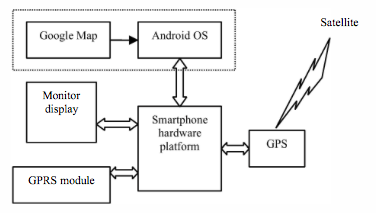
\includegraphics[clip]{paper-4}
  \caption*{图~4\hskip1em GPS导航系统的分析}
\end{figure}

\subsection*{3.4 病人信息的监控}

1) 原理分析:对于卧床的病人,医院需要监控他的各种信息,所以移动终端应该附有能够定时把病人病例信息传输到医院监控终端上以让医生能够诊断的能力。但这样的监控需要很多集成的通信模块和额外的医疗子模块。因为我们无法获取到所有硬件的需求,我们仅仅考虑常见的硬件资源:用相机的摄像头来获取视频监控功能,以提供最简单基础的监控信息。

2) 模块设计:这个模块包括视频收集模块、数据处理模块、图像展示模块。USB视频收集模块包括了USB摄像头、USB摄像头驱动两个模块。数据处理模块包括H.264解码库、收集和传输模块。整个工作流程可以参考图5。

\begin{figure}[h]
  \centering
  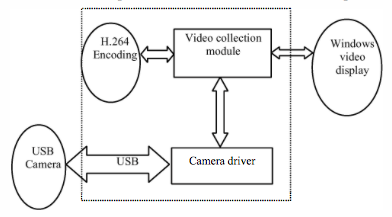
\includegraphics[clip]{paper-5}
  \caption*{图~5\hskip1em 监控系统的框架}
\end{figure}

\section*{4. 每个模块的关键部分}

\subsection*{4.1 病状和医疗方案模块中的数据获取}

1) 连接移动数据库:主要通过写程序调用移动数据库的接口来检查和组织病状和其医疗方案信息的特定分类。ListRecipe是这个系统中用来获取数据的一个子类$^{[6]}$,以下是一部分的接口代码:

\begin{lstlisting}[language=Java]
Cursor cur=getContentResolver().query(getlntent().getData(), PROJECTlON, sql, null, null);
\end{lstlisting}

2) 治疗方案的查询:通过安卓提供的元素接口,我们能够把界面展示和数据源结合来流畅展现对应的治疗方案、并且将模块安装到显示器上。ListRecipe也负责这一块,部分代码如下:

\begin{lstlisting}[language=Java]
SimpleAdapter adapter = new SimpleAdapter(this, fillMaps, R.layout.grid_item, from, to);
listView.setAdapter(adapter);
listView.setOnltemClickListener(this);
\end{lstlisting}

\subsection*{4.2 在医患非实时交流模块中的消息处理}

我们用来实现非实时通讯的基于安卓平台的移动端电子邮件主要包括的邮件发送和接收模块。系统需要处理文本或MIME(多目的电子邮件的拓展)的邮件类型。前者只包括两个部分:头(来自谁,发给谁,主题是什么)和主体(比如“你好X先生”之类)信息;而后者,信息被分成了若干个MIME分块,每个分块用一个特别的头信息来描述,比如常见的如表1,这样我们就需要对应的设置不同的类型。

\begin{table}[htbp]
\centering
\caption*{表A.1 不同类型}
\label{tab:ParametersForPandR}
\begin{tabular}[c]{lccc}
\toprule[1.5pt]
{\heiti 名称} & {\heiti 有效数值} & {\heiti 区分方法} \\\midrule[1pt]
MIME-版本 & 1.0 & MIME版本号 \\
内容-类型 & 文字,图片,语音,视频,应用,消息等 & 数据类型 \\
内容-传输-解码 & 7位或8位 & 数据解码类型 \\
\bottomrule[1.5pt]
\end{tabular}
\end{table}

\subsection*{4.3 病人地理位置信息模块的位置信息返回和分享}

我们通过编译继承于BroadcastReceiver的SMS\_Receiver类来完成位置定位需求信息的展示。在onReceiver函数中,先判断从监听的目的地是否是android.provider.Telephony.SMS\_RECEIVED$^{[6]}$。如果是,Bundle包的目的地会创建一个SMSMessage的数组。通过createFromPdu()函数以及SMS消息获取信息,然后通过getDisplayOriginationAddress()函数和getdisplayMessageBody()函数得到源码和信息内容如果信息包含LOCATION\_SMS,则通过以下两句代码开启位置服务:

\begin{lstlisting}[language=Java]
LocationManager mLocationManager = (Location_Manager)content.getSystemService(Context.LOCATION_SERVICE);
Location mLocation = getLocationProvider(mLocation_Manager);
\end{lstlisting}

然后经纬度的信息会通过一个SMS消息返回到移动收集用户,如果信息内容包含“LOCAL”,经纬度的信息会通过调用refreshMapView()函数来获取。

\subsection*{4.4 病人信息监控的视频收集}

在这个模块中我们使用数据报套接字(SOCK\_DGRAM)来达到视频数据的传递,因为这种方法在执行时比流套接字(SOCK\_STREAM)更快、成本更低。首先调用函数open("/dev/video0", 0\_RDWR)以打开视频设备。然后通过函数ioctl(fd, VIDIOCGCAP, \&rid\_cap)来获取类型video\_capability以读取摄像头图片的高度、宽度和其他相关信息。用mmap()内存匹配来获取视频图片。

\section*{5 总结}

在这里我们介绍了移动健康和安卓平台,设计了一套基于安卓的医患交互系统。在文章中我们分析了系统的应用需求和技术需求,并提升到了软件的层面,我们给出了基于有限硬件资源移动终端的医患交互模块主要部分的设计,并且确保了这些模块在安卓平台上是比较容易开发的$^{[8]}$。然而,系统依旧有一些缺点,比如如果物体在摄像头中变化比较大,展示模块的数据就会比较快的增长使得系统效率会降低。但由于安卓对于第三方应用的完全开放性,我相信未来会出现更好的服务,也会让移动健康这个领域有更好的性能。

\begin{center}
\section*{参考文献}
\end{center}

\begin{enumerate}[{$[$}1{$]$}]
\item R Wei, Z Yang. Design and implementation of doctor-patient interaction system based on android, ITME, 2012
\item Mark L.Murphy. The Busy Coder's Guide to Android Development. United States of America, Commons Ware, LLC., 2008
\item Justin\_luhui.baike.Baidu[EB/OL].[2010-10-12].
\item CHENG Chun-Iei, PAN Ze-qiang, "Research of chinese traditional medicine embeded information system based on android platform," Manufacturing Automation. pp 136-138. January 2011.
\item Shuiping Wei, Bangyan Ye, Zhiguang Fu, "Research on GPS Positioning Information Transfer Based on Wireless Network," 2007,28(6): 589-592.
\item Owens M., "Query Anything with SQLite," The World of Software Development, 2007, 32(12):24-28.
\item Jianxun Zhao, "Mobile Location Services Development and Implementation Based on Android Platform," Modern Business Trade Industry. pp 271-272. October 2010.
\item Chao-Tung Yang, Yen-Yu Chu, "Implementation of a Medical Information Service on Android Mobile Devices," New Trends in Information Science and Sercice Science, 2010(4):72-77.
\end{enumerate}

\begin{center}
\section*{书面翻译对应的原文索引}
\end{center}

\begin{enumerate}[{$[$}1{$]$}]
\item R Wei, Z Yang. Design and implementation of doctor-patient interaction system based on android, ITME, 2012
\end{enumerate}